\documentclass[tikz,border=3pt]{standalone}
\usepackage{amsmath,amssymb}
\usetikzlibrary{arrows.meta,calc}

\begin{document}
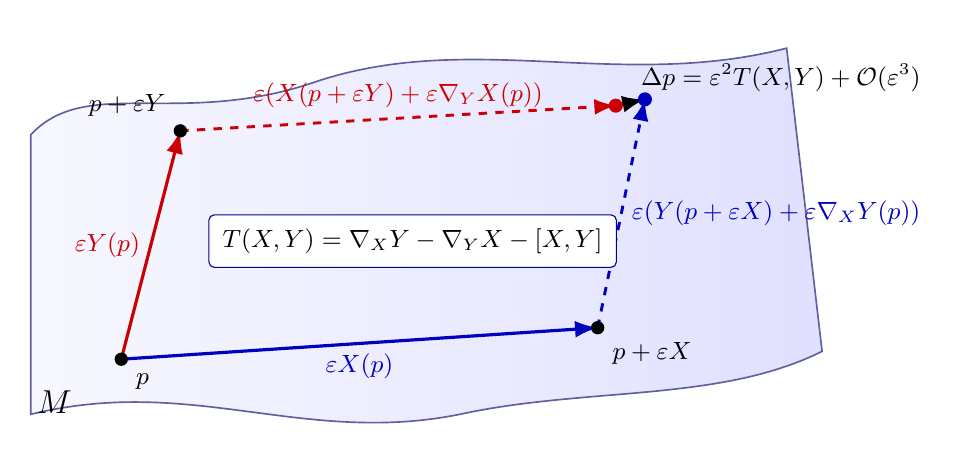
\begin{tikzpicture}[
  >=Latex,
  vector/.style={->,line width=1.15pt},
  transported/.style={->,line width=1.05pt,dashed},
  point/.style={circle,fill=black,inner sep=1.7pt},
  every node/.style={font=\small}
]
  \path[shade,left color=blue!3,right color=blue!12,draw=blue!25!gray,line width=.6pt]
    (0.15,0.55) .. controls (2.2,1.05) and (3.6,0.15) .. (5.6,0.55)
    .. controls (7.2,0.9) and (8.9,0.7) .. (10.2,1.35)
    -- (9.75,5.2)
    .. controls (7.6,4.65) and (5.7,5.45) .. (3.7,4.75)
    .. controls (2.0,4.2) and (0.85,4.85) .. (0.15,4.1) -- cycle;

  \coordinate (p) at (1.3,1.25);
  \coordinate (px) at (7.35,1.65);
  \coordinate (py) at (2.05,4.15);
  \coordinate (qblue) at (7.95,4.55);
  \coordinate (qred) at (7.58,4.47);

  \draw[vector,blue!75!black] (p) -- node[below] {$\varepsilon X(p)$} (px);
  \draw[transported,blue!75!black] (px) -- node[right] {$\varepsilon\!\left(Y(p+\varepsilon X)+\varepsilon\nabla_XY(p)\right)$} (qblue);
  \draw[vector,red!80!black] (p) -- node[left] {$\varepsilon Y(p)$} (py);
  \draw[transported,red!80!black] (py) -- node[above] {$\varepsilon\!\left(X(p+\varepsilon Y)+\varepsilon\nabla_YX(p)\right)$} (qred);
  \draw[vector,black] (qred) -- node[above right] {$\Delta p=\varepsilon^2T(X,Y)+\mathcal O(\varepsilon^3)$} (qblue);

  \node[point,label=below right:{$p$}] at (p) {};
  \node[point,label=below right:{$p+\varepsilon X$}] at (px) {};
  \node[point,label=above left:{$p+\varepsilon Y$}] at (py) {};
  \node[circle,fill=red!80!black,inner sep=1.8pt] at (qred) {};
  \node[circle,fill=blue!75!black,inner sep=1.8pt] at (qblue) {};

  \node[draw=blue!55!black,rounded corners=2pt,fill=white,inner sep=5pt]
    at (5.0,2.75) {$T(X,Y)=\nabla_XY-\nabla_YX-[X,Y]$};
  \node[font=\large] at (0.45,0.7) {$M$};
\end{tikzpicture}
\end{document}
